\subsection*{Liste des questions}
\begin{itemize}
  \item Q1 Veuillez me dire si vous êtes très intéressé(e), moyennement intéressé(e) ou pas du tout intéressé(e) par les découvertes scientifiques et les évolutions technologiques?\\
  \textit{[Trés intéressé / Moyennement / Pas du tout intéressé / NSP]}\\
  \item Q2 Je vais vous montrer deux images. Pour chacune d’entre elles, veuillez me dire dans quelle mesure elle correspond à l’idée que vous vous faites des robots.\\
  \textit{[très bien / plutôt bien / plutôt mal / très mal / NSP]}
\end{itemize}

\strut

\begin{minipage}{0.45\linewidth}
    \centering
    Robot, bras industriel\\
    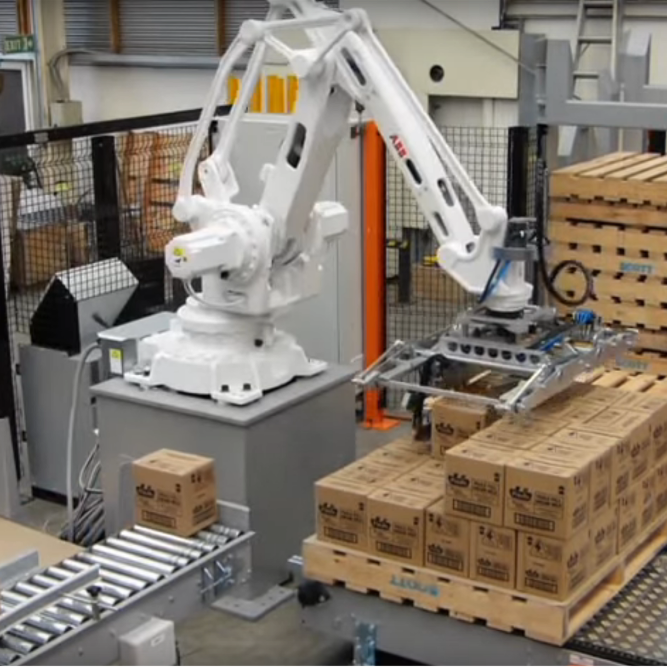
\includegraphics[width=0.95\linewidth]{Figures/Euro-QI2_1}
\end{minipage}
\hfill
\begin{minipage}{0.45\linewidth}
    \centering
    Robot, humanoïde\\
    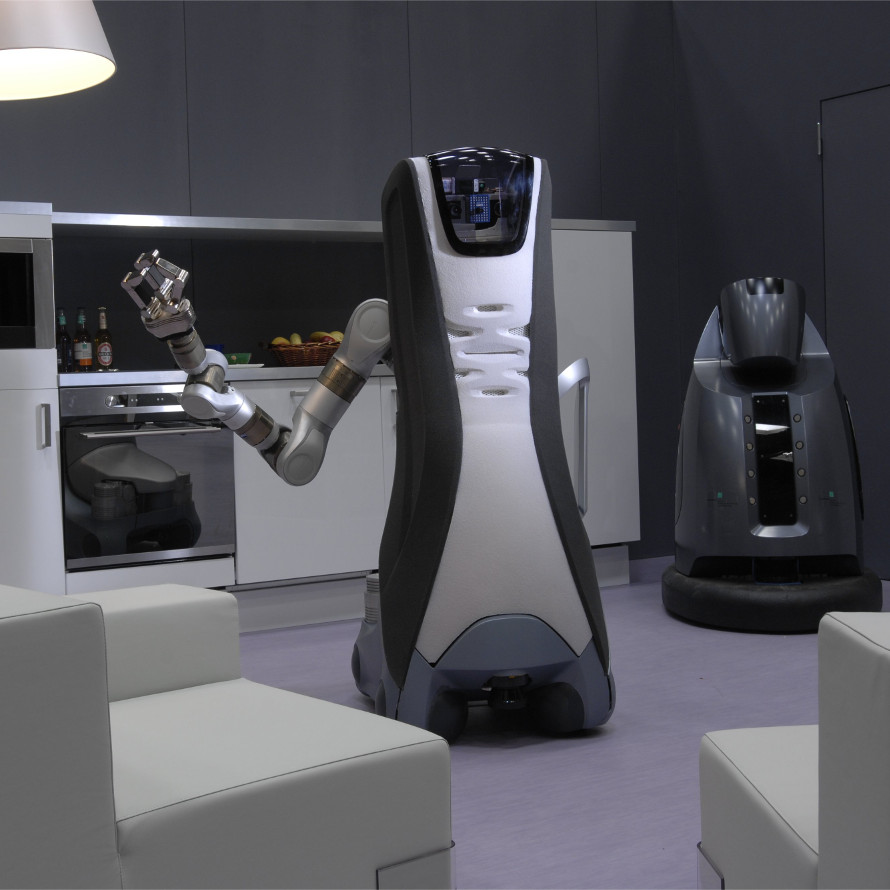
\includegraphics[width=0.95\linewidth]{Figures/Euro-QI2_2}
\end{minipage}

\strut

\begin{itemize}
  \item Q3 Avez-vous déjà utilisé, ou utilisez-vous actuellement, un robot de ce type à la maison ou sur votre lieu de travail (par ex. un robot aspirateur chez vous, ou un robot industriel au travail)? (PLUSIEURS REPONSES POSSIBLES)\\
  \textit{[oui à la maison / oui au travail / oui ailleurs / non / NSP]}\\
  \item Q4 De façon générale, avez-vous une image très positive, plutôt positive, plutôt négative ou très négative des robots?\\
  \textit{[très positive / plutôt positive / plutôt négative / très négative / NSP]}\\
  \item Q5 Veuillez me dire dans quelle mesure vous êtes d’accord ou pas d’accord avec les propositions suivantes concernant les robots.\\
  \textit{[tout à fait d'accord / pas du tout d'accord - échelle de 5 + NSP]}
    \begin{itemize}
    \item Les robots sont une bonne chose pour la société, parce qu’ils aident les gens.
    \item Les robots volent les emplois des gens.
    \item Les robots sont nécessaires parce qu’ils peuvent effectuer des tâches qui sont trop difficiles ou dangereuses pour les gens.
    \item Les robots sont un type de technologie qui nécessite d’être géré avec prudence.
    \item L’utilisation étendue des robots peut stimuler la création d’emplois dans l’UE.\\
    \end{itemize}
  \item Q6 Dans quels domaines pensez-vous que les robots devraient être utilisés en priorité ? (MAX. 3 REPONSES)\\
  \textit{La fabrication / Les soins de santé / Aux loisirs / Un usage domestique, comme le nettoyage / Les domaines militaire et de la sécurité / Les opérations de recherche et sauvetage / L’éducation / "La garde d’enfants, des personnes âgées et des personnes en situation de handicap" / L’exploration spatiale / L’agriculture / Le transport la logistique / Aucun}\\
  \item Q7 Et, au contraire, dans quels domaines pensez-vous que l’utilisation des robots devrait être rendue illégale? (MAX. 3 REPONSES)\\
  \textit{choix identique à Q6}\\
  \item Q8 Voici une liste de choses qui pourraient être faites par des robots. Pour chacune d’entre elles, pouvez-vous me dire ce que vous en pensez personnellement\\
  \textit{[tout à fait à l'aise / tout à fait mal à l'aise - échelle de notation à 9 points + Pas applicable + NSP]}
    \begin{itemize}
    \item Se faire opérer par un robot.
    \item Faire promener son chien par un robot.
    \item Être assisté(e) par un robot au travail (par ex. pour la production industrielle).
    \item Faire garder vos enfants ou vos parents âgés par un robot.\\
    \end{itemize}
  \item Q9 Selon vous, en Europe, quand les robots qui remplissent des tâches ménagères deviendront-ils une chose courante?\\
  \textit{[dans 5 ans / dans 10ans / dans 20 ans / dans plus de 20ans / jamais / c'est déjà une chose courante / NSP]}.
\end{itemize}

\section{Résultats EURO382}\label{pdf:euro_result}

\EuroGraph{Q1 Intérêt pour les découvertes scientifiques et les évolutions technologiques.}{QA1}

\vfill\strut

\EuroGraph{Q2-1 L'image [bras industriel] correspond à l’idée que vous vous faites des robots?}{QA2-1}

\EuroGraph{Q2-2 L'image [robot compagnons] correspond à l’idée que vous vous faites des robots?}{QA2-2}

\EuroGraph{Q3  Utilisez-vous un robot de ce type à la maison ou sur votre lieu de travail?}{QA3}

\EuroGraph{Q4 \textit{a priori} positif ou négatif sur les robots}{QA4}

\EuroGraph{Q5-1 Les robots sont une bonne chose pour la société, parce qu’ils aident les gens.}{QA5-1}

\EuroGraph{Q5-2 Les robots volent les emplois des gens.}{QA5-2}

\EuroGraph{Q5-3 Les robots sont nécessaires pour effectuer des tâches qui sont trop difficiles ou dangereuses pour les gens.}{QA5-3}

\EuroGraph{Q5-4 Les robots sont un type de technologie qui nécessite d’être géré avec prudence.}{QA5-4}

\EuroGraph{Q5-5 L’utilisation étendue des robots peut stimuler la création d’emplois dans l’UE.}{QA5-5}

\EuroGraph{Q6 Dans quels domaines pensez-vous que les robots devraient être utilisés en priorité ? (MAX. 3 REPONSES)}{QA6}

\EuroGraph{Q7 Dans quels domaines pensez-vous que l’utilisation des robots devrait être rendue illégale? (MAX. 3 REPONSES)}{QA7}

\EuroGraph{Q8-1 à l'aise / mal à l'aise de: Se faire opérer par un robot.}{QA8-1}

\EuroGraph{Q8-2 à l'aise / mal à l'aise de: Faire promener son chien par un robot.}{QA8-2}

\EuroGraph{Q8-3 à l'aise / mal à l'aise de: Être assisté(e) par un robot au travail (par ex. pour la production industrielle).}{QA8-3}

\EuroGraph{Q8-4 à l'aise / mal à l'aise de: Faire garder vos enfants ou vos parents âgés par un robot.}{QA8-4}

\EuroGraph{Q9 Selon vous, en Europe, quand les robots qui remplissent des tâches ménagères deviendront-ils une chose courante?}{QA9}
